
\chapter{Preface}
\label{cha:preface}


\section{Optimization problems}
\label{sec:optim-probl}

An \emph{optimization problem} is a pair $(ℱ,f)$, where $ℱ$ is a set, referred to as the set of \emph{feasible solutions},  and $f: ℱ ⟶ ℝ$ is a function, that is called the \emph{objective} or \emph{cost function}. The problem is to find an element $x ∈ ℱ$ such that
\begin{displaymath}
  f(x) ≥ f(y) \text{ holds for all } y ∈ ℱ. 
\end{displaymath}
Such an $x∈ ℱ$  is then an \emph{optimal solution} of the optimization problem.
Since the task is to find a global  maximum solution, we also write 
\begin{displaymath}
  \max \{ c(x) : x ∈ ℱ\}. 
\end{displaymath}

If the objective is to minimize $f(x)$ or, in other words, to find an $x ∈ ℱ$ with  
\begin{displaymath}
  f(x) ≤ f(y) \text{ for all } y ∈ ℱ,
\end{displaymath}
then this can be understood as the optimization problem $(ℱ,-f)$, since 
\begin{displaymath}
  -f(x) ≥ - f(y) \text{ for all } y ∈ ℱ \text{ if and only if }  f(x) ≤ f(y) \text{ for all } y ∈ ℱ. 
\end{displaymath}

\begin{example}
  \label{exe:1}
  From linear algebra we know the problem of maximizing  a
  \emph{quadratic form} $ x^T A x$ over the sphere
  $S^{(d-1)} = \{ x ∈ ℝ^d : \|x\| = 1 \} ⊆ ℝ^d$, where $A ∈ ℝ^{d×d}$ is a symmetric
  matrix.  Thus, in this case,   $ℱ = S^{(d-1)}$ and $f(x) = x^T A x$ and we write
  \begin{displaymath}
    \max\left\{ x^T A x : x ∈S^{(d-1)} \right\}. 
  \end{displaymath}
  If $v ∈ ℝ^d \setminus \{0\}$ is an eigenvector of $A$ corresponding to the
  maximal eigenvalue $λ_{\max} ∈ ℝ$ of $A$, then $v \ \|v\|$ is an optimal
  solution of the optimization problem.

  Following the discussion above, we see that an $x^* ∈ S^{(d-1)}$ is an optimal solution of
  \begin{displaymath}
    \min\left\{ x^T A x : x ∈S^{(d-1)} \right\} 
  \end{displaymath}
  if and only if $x^*$ is an optimal solution of
   \begin{displaymath}
    \max\left\{ x^T (-A) x : x ∈S^{(d-1)} \right\} . 
  \end{displaymath}
  We have seen that such an optimal solution is an eigenvector of $A$ corresponding to the minimal eigenvalue $λ_{\min}$ of $A$. 
\end{example}


\begin{example}
  \label{exe:4}
  

  A \emph{directed  graph} is a tuple $G = (V,A)$, where $V$ is a finite set of elements, called the
    \emph{vertices} of $G$ and  $A\subseteq(V\times V)$ is the set of
  \emph{arcs} of $G$. We denote an arc by its two defining nodes $(u,v) \in
  A$. The graph is \emph{weighted} if additionally equipped with a function $w: A ⟶ ℝ$ that maps the set of arcs to the reals. A \emph{simple path} is a finite sequence of \emph{distinct} vertices $P = v_1,v_2,\dots,v_k$  such that $(v_i,v_{i+1}) ∈A$ for each $i ∈ \{1,\dots,k-1\}$. The path is from $v_1$ to $v_k$ and the \emph{length} of the path $P$ is defined as
  \begin{displaymath}
    ℓ(P) = ∑_{i=1}^{k-1 } w(v_i,v_{i+1}). 
  \end{displaymath}


\begin{figure} \centering  
 \begin{tikzpicture}
	\begin{pgfonlayer}{nodelayer}
		\node [style=new style 0] (0) at (0, 5) {$a$};
		\node [style=new style 0] (1) at (2, 3) {$b$};
		\node [style=new style 0] (2) at (0, 2) {$d$};
		\node [style=new style 0] (3) at (2, 1) {$e$};
		\node [style=new style 0] (4) at (-1, 0) {$f$};
		\node [style=new style 0] (5) at (-2, 3) {$c$};
		\node [style=none] (6) at (1.25, 4.25) {$1$};
		\node [style=none] (7) at (-1.25, 4.25) {$3$};
		\node [style=none] (8) at (-0.25, 3.25) {$1$};
		\node [style=none] (9) at (-1.25, 2.25) {};
		\node [style=none] (10) at (-1.25, 2.25) {$0$};
		\node [style=none] (11) at (0.75, 1.5) {$2$};
		\node [style=none] (12) at (0.75, 0.25) {$1$};
		\node [style=none] (13) at (-1.75, 1.25) {$1$};
		\node [style=none] (14) at (2.25, 2.25) {$0$};
	\end{pgfonlayer}
	\begin{pgfonlayer}{edgelayer}
		\draw [style=edge] (0) to (1);
		\draw [style=edge] (0) to (2);
		\draw [style=edge] (1) to (3);
		\draw [style=edge] (2) to (3);
		\draw [style=edge] (3) to (4);
		\draw [style=edge] (0) to (5);
		\draw [style=edge] (5) to (4);
		\draw [style=edge] (5) to (2);
	\end{pgfonlayer}
\end{tikzpicture}
   
  \caption{Example of a weighted directed graph with $6$ nodes and $8$ arcs. A shortest path from $a$ to $f$ is  the node sequence $a,b,e,f$. Its length is equal to $2$.}
\label{fig:11}
\end{figure}

The \emph{shortest path problem} is now as follows. Given a  directed graph $G = (V,A)$  with non-negative weights $w: A ⟶ ℝ_+$  and two designated vertices $s$ and $t ∈V$, determine a path from $s$ to $t$ of minimal length. In our setting this is then the tuple $(ℱ,f)$, where $ℱ$ is the set of all paths from $s$ to $t$ in $G$ and $f(P)$ is equal to $-1$ times $ℓ(P)$. 

\end{example}

\subsection*{Linear programming}

Central to this course is the \emph{linear programming} or \emph{linear optimization} problem.  This is an optimization problem $(ℱ,f)$  where the set $ℱ$ is described by \emph{linear inequalities}
\begin{displaymath}
  ℱ = \{ x ∈ ℝ^n : Ax ≤ b\}, 
\end{displaymath}
where $A ∈ ℝ^{m ×n}$ is a matrix and $b ∈ ℝ^{m}$ is a vector. The objective function $f: ℝ^n ⟶ℝ$   is linear and of the form $f(x) = c^Tx$ for a given vector $c ∈ ℝ^n$.  


\begin{example}
  \label{ex-0:2}
    \begin{figure}
      \centering
      \tikzstyle{ipe stylesheet} = [
  ipe import,
  even odd rule,
  line join=round,
  line cap=butt,
  ipe pen normal/.style={line width=0.4},
  ipe pen heavier/.style={line width=0.8},
  ipe pen fat/.style={line width=1.2},
  ipe pen ultrafat/.style={line width=2},
  ipe pen normal,
  ipe mark normal/.style={ipe mark scale=3},
  ipe mark large/.style={ipe mark scale=5},
  ipe mark small/.style={ipe mark scale=2},
  ipe mark tiny/.style={ipe mark scale=1.1},
  ipe mark normal,
  /pgf/arrow keys/.cd,
  ipe arrow normal/.style={scale=7},
  ipe arrow large/.style={scale=10},
  ipe arrow small/.style={scale=5},
  ipe arrow tiny/.style={scale=3},
  ipe arrow normal,
  /tikz/.cd,
  ipe arrows, % update arrows
  <->/.tip = ipe normal,
  ipe dash normal/.style={dash pattern=},
  ipe dash dotted/.style={dash pattern=on 1bp off 3bp},
  ipe dash dashed/.style={dash pattern=on 4bp off 4bp},
  ipe dash dash dotted/.style={dash pattern=on 4bp off 2bp on 1bp off 2bp},
  ipe dash dash dot dotted/.style={dash pattern=on 4bp off 2bp on 1bp off 2bp on 1bp off 2bp},
  ipe dash normal,
  ipe node/.append style={font=\normalsize},
  ipe stretch normal/.style={ipe node stretch=1},
  ipe stretch normal,
  ipe opacity 10/.style={opacity=0.1},
  ipe opacity 30/.style={opacity=0.3},
  ipe opacity 50/.style={opacity=0.5},
  ipe opacity 75/.style={opacity=0.75},
  ipe opacity opaque/.style={opacity=1},
  ipe opacity opaque,
]
\definecolor{red}{rgb}{1,0,0}
\definecolor{blue}{rgb}{0,0,1}
\definecolor{green}{rgb}{0,1,0}
\definecolor{yellow}{rgb}{1,1,0}
\definecolor{orange}{rgb}{1,0.647,0}
\definecolor{gold}{rgb}{1,0.843,0}
\definecolor{purple}{rgb}{0.627,0.125,0.941}
\definecolor{gray}{rgb}{0.745,0.745,0.745}
\definecolor{brown}{rgb}{0.647,0.165,0.165}
\definecolor{navy}{rgb}{0,0,0.502}
\definecolor{pink}{rgb}{1,0.753,0.796}
\definecolor{seagreen}{rgb}{0.18,0.545,0.341}
\definecolor{turquoise}{rgb}{0.251,0.878,0.816}
\definecolor{violet}{rgb}{0.933,0.51,0.933}
\definecolor{darkblue}{rgb}{0,0,0.545}
\definecolor{darkcyan}{rgb}{0,0.545,0.545}
\definecolor{darkgray}{rgb}{0.663,0.663,0.663}
\definecolor{darkgreen}{rgb}{0,0.392,0}
\definecolor{darkmagenta}{rgb}{0.545,0,0.545}
\definecolor{darkorange}{rgb}{1,0.549,0}
\definecolor{darkred}{rgb}{0.545,0,0}
\definecolor{lightblue}{rgb}{0.678,0.847,0.902}
\definecolor{lightcyan}{rgb}{0.878,1,1}
\definecolor{lightgray}{rgb}{0.827,0.827,0.827}
\definecolor{lightgreen}{rgb}{0.565,0.933,0.565}
\definecolor{lightyellow}{rgb}{1,1,0.878}
\definecolor{black}{rgb}{0,0,0}
\definecolor{white}{rgb}{1,1,1}
\begin{tikzpicture}[ipe stylesheet]
  \filldraw[ipe pen heavier, -{>[ipe arrow large]}, fill=lightgray]
    (256, 704)
     -- (192, 640)
     -- (320, 640)
     -- cycle;
  \draw[ipe pen heavier, -{>[ipe arrow large]}]
    (128, 640)
     -- (384, 640);
  \draw[ipe pen heavier, -{>[ipe arrow large]}]
    (256, 576)
     -- (256, 768);
  \node[ipe node]
     at (384, 624) {$x_1$};
  \node[ipe node]
     at (272, 768) {$x_2$};
  \node[ipe node]
     at (304, 624) {$(1,0)$};
  \node[ipe node]
     at (176, 624) {$(-1,0)$};
  \node[ipe node]
     at (256, 720) {$(0,1)
$};
\end{tikzpicture}
  
      \caption{The set $ℱ$ in example~\ref{ex-0:2}}. 
      \label{fig:10}
    \end{figure}

  Let $A ∈ ℝ^{3 ×2}$ be the matrix
  \begin{displaymath}
    A =
    \begin{pmatrix}
      -1 & 1 \\
      1 & 1 \\
      0 & -1 
    \end{pmatrix}
  \end{displaymath}
  and $b ∈ ℝ^3$ be the vector
  \begin{displaymath}
    b =
    \begin{pmatrix}
      1 \\ 1 \\ 0
    \end{pmatrix}
  \end{displaymath}
  The set $ℱ ⊆ ℝ^2$ is the set of all points $(x_1,x_2)^T ∈ ℝ^2$ in the plane that satisfy all three inequalities
  \begin{displaymath}
    -x_1+ x_2 ≤1, \,  x_1+ x_2 ≤1, \text{ and } x_2 ≥0. 
  \end{displaymath} This set $ℱ$ is the triangle depicted in Figure~\ref{fig:10}. 
  If we set the objective function as $f(x) = x_2$, then $x = (0,1)^T$ is an optimal solution.   
\end{example}
The linear optimization problem is one of the most important types of mathematical optimization problems. It has numerous applications in science and engineering and, in particular, modern fields like \emph{machine learning}. In fact, the shortest 

In this course, we will learn  the theory of linear optimization and develop \emph{efficient algorithms} to solve linear programming problems. This means that we do not content ourselves with an algorithm that is correct, but we want this algorithm to be capable to solve large scale problems within a short time. 




\section{Certificates}
\label{sec:certificates}


A central topic in linear algebra is the theory around  linear equations 
\begin{equation} 
\label{p:eq:1}
  A \, x = b
\end{equation}
where $A ∈ ℝ^{m×n}$ is a given matrix and $b ∈ ℝ^m$ is a given vector. Every student of mathematics learns learns to appreciate \emph{Gaussian elimination} which transforms the system~\eqref{p:eq:1}  into an equivalent system  
\begin{displaymath}
  {A}' x = {b}'
\end{displaymath}
that is in row-echelon form. This means that ${A}' ∈ ℝ^{m×n}$ is such that 
  for each $i ∈ \{ 1,\dots , m-1\}$
  \begin{displaymath}
    \min\{ j : {a}'_{ij} \neq 0\} <  \min\{ j : {a}'_{i+1j} \neq 0\},
  \end{displaymath}
see Figure~\ref{fig:8}. 


\begin{figure}
  \centering
 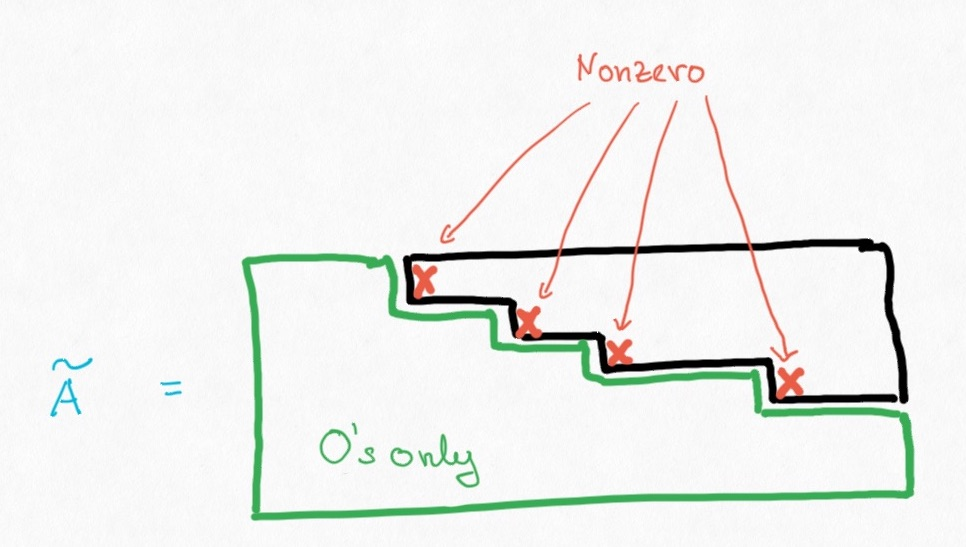
\includegraphics[height=5cm]{figures/RowEchelon.jpg}
  \caption{A schematic image of a matrix in row-echelon form} 
\label{fig:8}
\end{figure}


The system~\eqref{p:eq:1} has a solution if and only if ${b}'$ has only zero's in those components that correspond to the zero-rows of ${A}'$ and a solution is readily computed. In fact, Gaussian elimination also provides an invertible matrix $Q ∈ ℝ^{m ×m}$ such that $Q\cdot A = {A}'$ and $Q \cdot b = {b}'$. If the $i$-th component of ${b}'$ is nonzero and the $i$-th row of ${A}'$ consists of zeros only, then with $q$ being the column vector corresponding to the $i$-th row of $Q$ one has 
\begin{displaymath}
  q^T A = 0 \text{ and } q^Tb \neq 0. 
\end{displaymath}
Thus there is a convenient \emph{certificate} of the fact that \eqref{p:eq:1} is not solvable. 


\begin{theorem}
  \label{thr:8}
  A linear system~\eqref{p:eq:1} is not solvable if and only if there exists a vector $q ∈ ℝ^m$ such that 
  \begin{displaymath}
    q^T A = 0 \text{ and } q^T b \neq 0. 
  \end{displaymath}
\end{theorem}

In this course, we will now also deal with systems of \emph{linear inequalities} 
\begin{equation}
  \label{p:ineq}
  A \,x ≤ b,
\end{equation}
where $A ∈ ℝ^{m × n}$ and $b ∈ ℝ^m$. A \emph{solution} to such a system is a vector $x^* ∈ ℝ^m$ such that
\begin{equation}
  \label{p:sol}
 \text{for each } i=1,\dots,m \quad : \quad   a_{i1} x^*_1 + \cdots + a_{in} x^*_n \leq b_i.  
\end{equation}
If a solution exists, the system~\eqref{p:ineq} is called \emph{feasible} otherwise it is called \emph{infeasible}. 
We will ask analogous questions for  systems of linear inequalities as we did for linear equations. Can we efficiently find a solution of~\eqref{p:ineq}?  Is there a simple certificate to convince somebody of the infeasibility of \eqref{p:ineq}? 

To shed a bit of light on this second question, let us consider a vector $λ ∈ ℝ^m_{≥0}$. If $x^*$ is a solution, then $x^*$ also satisfies the inequality 
\begin{equation}
  \label{p:impli}
  λ^T A \, x ≤ λ^T b.
\end{equation}
If there exists a $λ \in ℝ^m_{≥0}$ such that 
\begin{equation}
  \label{p:Farkas} 
  λ^T A = 0^T \text{ and } λ^T b = -1,
\end{equation}
then this $λ$ \emph{certifies} that~\eqref{p:ineq} is infeasible. In the case of infeasibility, can such a $λ≥0$ always be found? Among the many results presented in  this course,  we will show that the answer is ``yes''. 
\begin{theorem}[Farkas' lemma]
  \label{thr:7}
  A system of linear inequalities~\eqref{p:ineq} is infeasible if and only if there exists a $λ ∈ ℝ^m_{≥0}$ such that 
  \begin{displaymath}
    λ^T A = 0 \text{ and } λ^T b = -1.
  \end{displaymath}
\end{theorem}


\bigskip

More generally, we will learn about certificates of optimality of linear optimization problems. Lets consider again example~\ref{exe:1}. How can we certify that $x^* = (0,1)^T$ is an optimal solution of the linear program.

Each point $x^*$ in $ℱ$ must satisfy the first two linear inequalities
\begin{displaymath}
  -x_1 + x_2 ≤ 1 \text{ and }  x_1 + x_2 ≤ 1. 
\end{displaymath}
But then such an $x^*$ satisfies also the \emph{sum} of these two inequalities
\begin{displaymath}
   (-x_1 + x_2) + (x_1 + x_2) ≤ 1  +1 
 \end{displaymath}
 which simplifies to
 \begin{displaymath}
x_2 ≤1. 
 \end{displaymath}
 But $x_2$ is the objective function. We have just shown that the objective function value of any point is at most $1$. Since this objective function value at $x^* = (0,1)^T$ is \emph{equal} to one, we have certified optimality of $x^*$.

 \bigskip

The general theory that makes certification of optimility possible for linear optimization is the theory of \emph{duality}. It is a rich theory with many other applications in discrete mathematics. We will touch upon many of them.

 




\section*{Exercises}

\begin{enumerate}[1)]
\item Provide a certificate as in Theorem~\ref{thr:8} of the unsolvability of the linear equation 
  \begin{displaymath}
    \begin{pmatrix}
      2 & 1 & 0 \\
      5 & 4 & 1 \\
      7 & 5 & 1
    \end{pmatrix} \,
    \begin{pmatrix}
      x_1 \\ x_2 \\ x_3 
    \end{pmatrix} =
    \begin{pmatrix}
      1\\2\\4
    \end{pmatrix}
  \end{displaymath}
\item Show the ``if'' direction of the Farkas' lemma (Theorem~\ref{thr:7}). 
\item The directed graph $G = (V,A)$ is \emph{complete}, if $A = \{(u,v) : u≠v ∈ V\}$. Let $s ≠ t ∈V$ be two designated vertices. How many directed paths connect $s$ and $t$ in $G$? Find a formula with parameter $n = |V|$. 
\item Let $G = (V,A)$ be a directed graph and $s,t ∈ V$ be two designated vertices. For a vertex $v ∈ V$ we let
  \begin{displaymath}
    δ^+(v) = \{ (u,v) : u ∈ V, \, (u,v) ∈A\} \text{ and } δ^i(v) = \{ (v,u) : u ∈ V, \, (v,u) ∈A\}
  \end{displaymath}
  the \emph{arcs entering} and \emph{leaving} $u$ respectively.  Consider the following inequalities
  \begin{equation} 
    \begin{array}{rclc}      \displaystyle 
    ∑_{a ∈ δ^+(v) } x_a -  ∑_{a ∈ δ^-(v) } x_a & = &  0 & \, \quad v ∈ V \setminus \{s,t\} \\ \displaystyle 
      ∑_{a ∈ δ^+(s) } x_a -  ∑_{a ∈ δ^-(s) } x_a & = &  -1 & \\
      \displaystyle 
      ∑_{a ∈ δ^+(t) } x_a -  ∑_{a ∈ δ^-(t) } x_a & = &  1 & \\
      x_a &≥& 0 & a ∈A.
    \end{array}
    \label{eq:1}
  \end{equation}
  
  \begin{enumerate}[a)] 
  \item Consider the following digraph with $s$ and $t$ and a partial assignment of arc variables. Can this partial assignment be completed to a feasible solution satisfying the inequalities~\eqref{eq:1}? If yes, complete the assignment.
    \begin{center}
          \begin{tikzpicture}
	\begin{pgfonlayer}{nodelayer}
		\node [style=new style 0] (0) at (0, 4) {$s$};
		\node [style=new style 0] (1) at (0, -4) {$t$};
		\node [style=new style 0] (2) at (3, 2) {};
		\node [style=new style 0] (3) at (-3, 2) {};
		\node [style=new style 0] (4) at (0, 0) {};
		\node [style=new style 0] (5) at (3, -2) {};
		\node [style=new style 0] (6) at (-3, -2) {};
		\node [style=none] (7) at (-1.75, 3.5) {$.5$};
		\node [style=none] (8) at (2.25, 3.75) {$.75$};
		\node [style=none] (9) at (0.75, 2.5) {};
		\node [style=none] (10) at (1.25, 1.25) {$.25$};
		\node [style=none] (11) at (2.25, 0.25) {};
		\node [style=none] (12) at (-3.75, 0) {};
		\node [style=none] (13) at (-1.75, -3.25) {};
		\node [style=none] (14) at (0.5, -2) {$0$};
		\node [style=none] (15) at (2.25, -1) {};
		\node [style=none] (16) at (1.75, -3.25) {};
		\node [style=none] (17) at (-1, 1.25) {.25};
	\end{pgfonlayer}
	\begin{pgfonlayer}{edgelayer}
		\draw [style=edge] (0) to (3);
		\draw [style=edge] (3) to (4);
		\draw [style=edge, bend left] (0) to (2);
		\draw [style=edge, bend left=45] (2) to (4);
		\draw [style=edge, bend left] (2) to (0);
		\draw [style=edge, bend left, looseness=1.25] (4) to (2);
		\draw [style=edge] (3) to (6);
		\draw [style=edge] (4) to (1);
		\draw [style=edge] (4) to (5);
		\draw [style=edge] (6) to (1);
		\draw [style=edge] (5) to (1);
	\end{pgfonlayer}
\end{tikzpicture}
   
    \end{center}
\item Show the following for a digraph $G = (V,A)$ with $s,t ∈ V$: If there is a path connecting $s$ and $t$ in $G$, then the system of inequalities~\eqref{eq:1} has a feasible solution
  \item (*)  Show the following for a digraph $G = (V,A)$ with $s,t ∈ V$: If  the system of inequalities~\eqref{eq:1} has a feasible solution, then  there is a path connecting $s$ and $t$ in $G$. 
   \end{enumerate}
  
\end{enumerate}



 

%%% Local Variables: 
%%% mode: latex
%%% TeX-master: "lecture"
%%% End: 
